% !TeX program = pdflatex
% =============================================================
% Public Economics -- Lecture 2
% Theoretical Tools of Public Finance
% Based on: Gruber, J. "Public Finance and Public Policy", Ch. 2
%           Stantcheva, S. "Lecture 2: Theoretical Tools for Public
%           Economics" (Harvard EC2450A, Fall 2022)
% Austrian institutional and empirical context added for WU Vienna.
% =============================================================
\documentclass[11pt,aspectratio=169]{beamer}

\usetheme{metropolis}
\usepackage[utf8]{inputenc}
\usepackage[T1]{fontenc}
\usepackage{lmodern}
\usepackage{booktabs}
\usepackage{array}
\usepackage{textcomp}
\usepackage{siunitx}
\usepackage{tikz}
\usepackage{pgfplots}
\pgfplotsset{compat=1.18}
\usepackage{pgf-pie}
\usetikzlibrary{positioning,arrows.meta,calc}

% ----------------------------------------------------------------
% Colors: WU Vienna blue as primary accent
% ----------------------------------------------------------------
\definecolor{wublue}{HTML}{003D7C}
\definecolor{wulight}{HTML}{4F8FC4}
\definecolor{wugray}{HTML}{5C6670}
\definecolor{wured}{HTML}{B0202E}
\definecolor{wugreen}{HTML}{4C8C6B}
\definecolor{wuyellow}{HTML}{D9A441}
\setbeamercolor{palette primary}{bg=wublue,fg=white}
\setbeamercolor{frametitle}{bg=wublue,fg=white}
\setbeamercolor{progress bar}{fg=wublue,bg=wulight!30}
\setbeamercolor{alerted text}{fg=wured}

\setbeamertemplate{frame footer}{Theoretical Tools of Public Finance}
\setbeamertemplate{footline}[frame number]

\title{Public Economics}
\subtitle{Lecture 2 \(\cdot\) Theoretical Tools of Public Finance}
\author{Dr. Shushanik Margaryan}
\institute{WU Vienna University of Economics and Business}
\date{Winter Term}

% Source note command for footnote-style citations on data slides
\newcommand{\srcnote}[1]{{\footnotesize\color{wugray}Source: #1}}

\begin{document}

% =============================================================
\begin{frame}
  \titlepage
\end{frame}

% =============================================================
\begin{frame}{Today's Questions}
  \begin{itemize}
  	\item In this lecture we will review microeconomic concepts that most of you should be familiar with
    \item Utility function, budget constraints, indifference curves, etc.
 
    \item What is the theoretical effect of raising --- or cutting --- Austria's minimum-income support (\alert{Sozialhilfe}) on economic efficiency?
  \end{itemize}


\end{frame}

\begin{frame}{Outline}
  \tableofcontents
\end{frame}

\begin{frame}{Theoretical vs.\ Empirical Tools}
  \begin{block}{Theoretical tools}
    The set of tools designed to understand the \emph{mechanics} behind economic decision making --- graphical and mathematical models of utility maximization subject to constraints.
  \end{block}
  \begin{block}{Empirical tools}
    The set of tools designed to \emph{analyze data} and answer the questions raised by theoretical analysis (the subject of Lecture 3).
  \end{block}
  \vspace{0.5em}
  \centering
  Theory tells us the \emph{direction} of an effect; data tells us its \emph{size}. We need both.
\end{frame}

% =============================================================
\section{2.1 Constrained Utility Maximization}

\begin{frame}{Utility Functions}
  \begin{block}{Utility function}
    A mathematical mapping of an individual's consumption choices into a level of well-being: $U = u(X_1, X_2, \ldots)$.
  \end{block}
  \begin{itemize}
    \item Consumers are assumed to undertake \textbf{constrained utility maximization}: maximize well-being subject to available resources.
    \item Key assumption: \textbf{non-satiation} (``more is better'') --- more of a good is always at least as good as less.
  \end{itemize}
  \vspace{0.5em}
  \centering
  \textbf{Running example:} Lena, a WU student, choosing between \emph{coffees at the Kaffeehaus} ($C$) and \emph{cinema visits} ($M$).
\end{frame}

\begin{frame}{Indifference Curves}
  \footnotesize
  \begin{columns}[T]
    \begin{column}{0.45\textwidth}
      \begin{block}{Indifference curve}
        All bundles of goods that leave an individual equally well off.
      \end{block}
      \begin{itemize}
        \item Bundle $A$: 2 coffees, 1 cinema visit
        \item Bundle $B$: 1 coffee, 2 cinema visits
        \item Bundle $C$: 2 coffees, 2 cinema visits
      \end{itemize}
      Lena is indifferent between $A$ and $B$, but strictly prefers $C$ to both (more of everything).
    \end{column}
    \begin{column}{0.55\textwidth}
      \begin{center}
      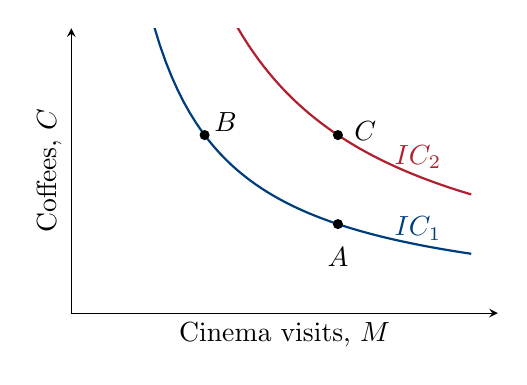
\begin{tikzpicture}
        \begin{axis}[
          width=7cm, height=5.2cm,
          xmin=0, xmax=3.2, ymin=0, ymax=3.2,
          xlabel={Cinema visits, $M$}, ylabel={Coffees, $C$},
          axis lines=left,
          ticks=none,
          ]
          \addplot[wublue, thick, domain=0.35:3, samples=60] {2/x};
          \addplot[wured, thick, domain=0.7:3, samples=60] {4/x};
          \node[wublue] at (axis cs:2.6,0.95) {$IC_1$};
          \node[wured] at (axis cs:2.6,1.75) {$IC_2$};
          \addplot[only marks, mark=*, mark size=1.6pt, black] coordinates {(1,2) (2,1) (2,2)};
          \node[anchor=west] at (axis cs:1,2.15) {$B$};
          \node[anchor=north] at (axis cs:2,0.85) {$A$};
          \node[anchor=west] at (axis cs:2.05,2.05) {$C$};
        \end{axis}
      \end{tikzpicture}
      \end{center}
    \end{column}
  \end{columns}
  Two properties (both from ``more is better''): (1) higher indifference curves are preferred; (2) indifference curves always slope downward.
\end{frame}

\begin{frame}{Marginal Utility}
  \begin{block}{Marginal utility}
    The additional utility from consuming one more unit of a good: $MU_1 = \partial u / \partial X_1$.
  \end{block}
  \begin{itemize}
    \item Example: $U = \sqrt{C \times M}$ (holding $C=2$ fixed). Moving from 0 to 1 cinema visit raises $U$ from 0 to $\sqrt{2}=1.41$; from 1 to 2 visits, $U$ rises only to $\sqrt{4}=2$ (a gain of $0.59$); from 2 to 3, the gain is only $0.45$.
    \item This is \textbf{diminishing marginal utility}: each additional unit of a good raises utility by less than the previous unit.
  \end{itemize}
\end{frame}

\begin{frame}{Aside: Does Marginal Utility Always Diminish?}
  \begin{alertblock}{Not for addictive goods}
    \end{alertblock}
    Becker \& Murphy (1988), ``A Rational Theory of Addiction'': today's utility from consuming a good can depend on \emph{past} consumption of it --- you build a habit.

  \begin{itemize}
    \item The more you have already consumed, the more you enjoy (or ``need'') consuming more --- the opposite of diminishing MU.
    \item This is a leading theoretical framework for taxing tobacco, alcohol, and sugar: if consumers systematically under-weigh future harm, corrective taxes can improve welfare beyond just correcting externalities.
  \end{itemize}
\end{frame}

\begin{frame}{Marginal Rate of Substitution}
  \begin{block}{Marginal rate of substitution (MRS)}
    The rate at which a consumer is willing to trade one good for another; equals (minus) the slope of the indifference curve: $MRS_{C,M} = MU_M / MU_C$.
  \end{block}
  \begin{itemize}
    \item For $U=\sqrt{C \times M}$: $MRS_{C,M} = C/M$.
    \item \textbf{Diminishing MRS}: as Lena has more cinema visits and fewer coffees, she is willing to give up less and less coffee for one more visit.
  \end{itemize}
  \vspace{0.3em}
  \centering
  Diminishing MRS is exactly why indifference curves are \emph{convex} (bowed toward the origin).
\end{frame}

\begin{frame}{Budget Constraints}
  \begin{block}{Budget constraint}
    All combinations of goods an individual can afford, spending her entire income: $P_C \, C + P_M \, M = Y$.
  \end{block}
  \begin{itemize}
    \item Suppose a Kaffeehaus coffee costs \texteuro{}4, a cinema ticket costs \texteuro{}8, and Lena's monthly ``fun budget'' is \texteuro{}96.
    \item Maximum coffees (0 cinema): $96/4 = 24$. Maximum cinema visits (0 coffee): $96/8 = 12$.
    \item Slope of the budget line: $-P_M/P_C = -8/4 = -2$ --- each extra cinema visit costs 2 coffees.
  \end{itemize}
\end{frame}

\begin{frame}{Constrained Choice: The Tangency Condition}
  \begin{columns}[T]
    \begin{column}{0.42\textwidth}
      \begin{itemize}
        \item Lena's optimal bundle is where her highest reachable indifference curve is \textbf{tangent} to her budget line.
        \item At that point: $MRS_{C,M} = P_M/P_C$.
        \item With $U=\sqrt{C\times M}$ and this budget: optimum is $M=6$, $C=12$ (she splits her \texteuro{}96 evenly: \texteuro{}48 on each good).
      \end{itemize}
    \end{column}
    \begin{column}{0.58\textwidth}
      \begin{center}
      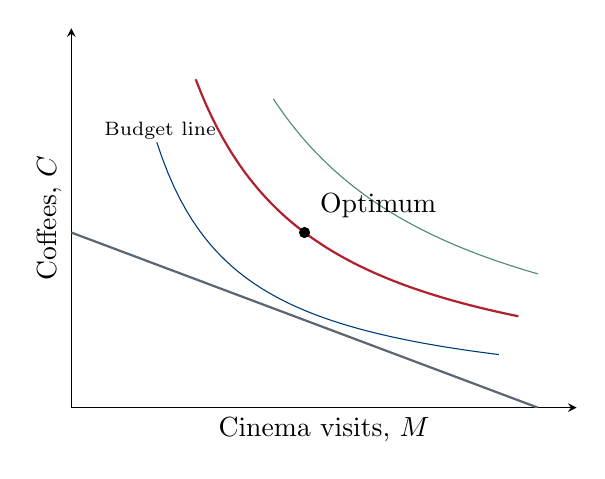
\begin{tikzpicture}
        \begin{axis}[
          width=8cm, height=6.4cm,
          xmin=0, xmax=13, ymin=0, ymax=26,
          xlabel={Cinema visits, $M$}, ylabel={Coffees, $C$},
          axis lines=left,
          ticks=none,
          ]
          \addplot[wugray, thick, domain=0:12] {96/8 - x};
          \addplot[wublue, thin, domain=2.2:11, samples=60] {40/x};
          \addplot[wured, thick, domain=3.2:11.5, samples=60] {72/x};
          \addplot[wugreen, thin, domain=5.2:12, samples=60] {110/x};
          \node[anchor=west, font=\scriptsize] at (axis cs:0.6,19) {Budget line};
          \addplot[only marks, mark=*, mark size=1.8pt, black] coordinates {(6,12)};
          \node[anchor=south west] at (axis cs:6.15,12.3) {Optimum};
        \end{axis}
      \end{tikzpicture}
      \end{center}
    \end{column}
  \end{columns}
\end{frame}

\begin{frame}{Income and Substitution Effects}
  Suppose the price of cinema tickets rises. This has two distinct effects on demand:
  \begin{block}{Substitution effect}
    Holding utility constant, a relative price rise \emph{always} causes less consumption of that good.
  \end{block}
  \begin{block}{Income effect}
    A price rise makes the consumer effectively poorer, typically reducing consumption of \emph{all} normal goods.
  \end{block}
  \vspace{0.3em}
  \centering
  For a normal good, both effects push demand in the \emph{same} direction --- toward less of the good whose price rose.
\end{frame}

%\begin{frame}{Decomposing a Price Change}
%  \begin{center}
%  \begin{tikzpicture}
%    \begin{axis}[
%      width=11cm, height=6cm,
%      xmin=0, xmax=14.5, ymin=0, ymax=7,
%      xlabel={Cinema visits, $M$}, ylabel={Coffees, $C$},
%      axis lines=left,
%      ticks=none,
%      ]
%      \addplot[wugray, thick] coordinates {(0,6) (12,0)};
%      \addplot[wugray, thick, dashed] coordinates {(0,6) (6,0)};
%      \addplot[wugreen, thick, dashed] coordinates {(0,6.9) (9,0)};
%      \addplot[wublue, thin, domain=1.6:9.5, samples=60] {18/x};
%      \addplot[wured, thin, domain=2:9.5, samples=60] {9/x};
%      \addplot[only marks, mark=*, mark size=1.8pt, black] coordinates {(6,3) (4.24,4.24) (3,3)};
%      \node[anchor=south west] at (axis cs:6.1,3.1) {$A$};
%      \node[anchor=south west] at (axis cs:4.34,4.34) {$B$};
%      \node[anchor=north east] at (axis cs:2.9,3.1) {$C$};
%      \node[anchor=west] at (axis cs:12.1,0.05) {$BC_1$};
%      \node[anchor=west] at (axis cs:6.1,0.05) {$BC_2$};
%      \node[anchor=west] at (axis cs:9.1,0.55) {$BC_g$};
%      \draw[<->, wured] (axis cs:3,1.6) -- (axis cs:4.24,1.6) node[midway, above, font=\scriptsize]{Income};
%      \draw[<->, wublue] (axis cs:4.24,2.2) -- (axis cs:6,2.2) node[midway, above, font=\scriptsize]{Substitution};
%    \end{axis}
%  \end{tikzpicture}
%  \end{center}
%  \centering \small
%  Cinema price rises: $A \to C$ overall. $A \to B$ (holding utility at $IC_1$) isolates the \emph{substitution effect}; $B \to C$ isolates the \emph{income effect}.
%\end{frame}

\begin{frame}{Normal vs.\ Inferior Goods}
  \begin{block}{Normal good}
    Demand \emph{increases} with income (most goods).
  \end{block}
  \begin{block}{Inferior good}
    Demand \emph{decreases} with income.
  \end{block}
  \vspace{0.5em}
 
Do you have an example of an inferior good?
 
\end{frame}

% =============================================================
\section{2.2 Putting the Tools to Work: Sozialhilfe and Labor Supply}

\begin{frame}{Austria's Sozialhilfe (Minimum Income Support)}
  \begin{itemize}
    \item Since the 2019 \emph{Sozialhilfe-Grundsatzgesetz}, Austria's means-tested minimum income sets \textbf{maximum} rates (\emph{Höchstsätze}), not guaranteed minimums, with details varying by \emph{Land}.
    \item Maximum monthly rate for a single adult/single parent (2024): \(\approx\)\texteuro{}1{,}156. Average \emph{actual} payment to single adults: \(\approx\)\texteuro{}766/month.
    \item A 2019 reform introduced the \emph{Freibetrag}: up to 35\% of net earnings are disregarded (not counted against the benefit) for up to 12 months when a recipient starts working.
  \end{itemize}
 
 
 
\end{frame}

\begin{frame}{The Consumption--Leisure Trade-off}
  \begin{itemize}
    \item Suppose Julia, a single parent, can work up to 2{,}000 hours/year at a wage of \texteuro{}10/hour, with no other income and no Sozialhilfe.
    \item Each hour of leisure ``costs'' her \texteuro{}10 in forgone wages (opportunity cost).
    \item Her budget constraint: maximum \texteuro{}20{,}000/year in consumption (0 leisure) or 2{,}000 hours of leisure (\texteuro{}0 consumption); slope $=-10$.
  \end{itemize}
\end{frame}

\begin{frame}{Adding Sozialhilfe to the Budget Constraint}
  \begin{center}
  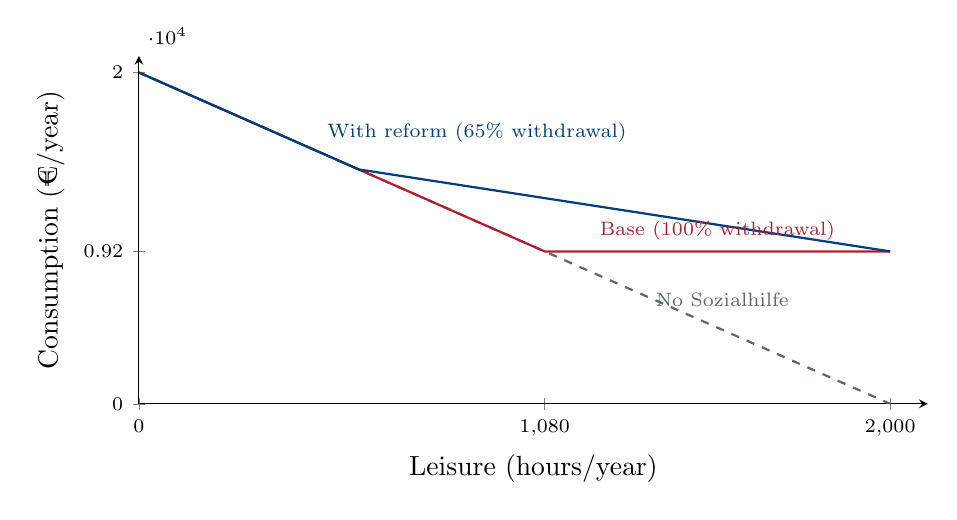
\begin{tikzpicture}
    \begin{axis}[
      width=11.6cm, height=6cm,
      xmin=0, xmax=2100, ymin=0, ymax=21000,
      xlabel={Leisure (hours/year)}, ylabel={Consumption (\texteuro/year)},
      axis lines=left,
      xtick={0,1080,2000},
      ytick={0,9200,20000},
      tick label style={font=\scriptsize},
      ]
      \addplot[wugray, thick, dashed] coordinates {(0,20000) (2000,0)};
      \addplot[wured, thick] coordinates {(0,20000) (1080,9200) (2000,9200)};
      \addplot[wublue, thick] coordinates {(0,20000) (585,14150) (2000,9200)};
      \node[anchor=west, font=\scriptsize, wugray] at (axis cs:1350,6300) {No Sozialhilfe};
      \node[anchor=south, font=\scriptsize, wured] at (axis cs:1540,9250) {Base (100\% withdrawal)};
      \node[anchor=south, font=\scriptsize, wublue] at (axis cs:900,15200) {With reform (65\% withdrawal)};
    \end{axis}
  \end{tikzpicture}
  \end{center}
  \centering \small
  Without any earnings disregard, Julia's net return to work is \texteuro{}0 until she earns her way off Sozialhilfe entirely --- a pure ``welfare trap.''
\end{frame}

\begin{frame}{The Wiedereinsteigerfreibetrag: A Real Reduction-Rate Experiment}
  \begin{itemize}
    \item \textbf{Base regime}: 100\% benefit-reduction rate. Every euro earned reduces Sozialhilfe by one euro --- net return to work is \texteuro{}0 (flat budget segment).
    \item \textbf{Reform regime}: 35\% of net earnings disregarded $\Rightarrow$ effective reduction rate \(\approx\)65\%. Net return to work rises to \texteuro{}3.50 per hour (slope $-3.5$ instead of flat).
  \end{itemize}
\end{frame}

\begin{frame}{Predicted Effects on Labor Supply}
  \begin{itemize}
    \item Cutting the reduction rate (100\% $\to$ 65\%) makes work pay more --- a pure \textbf{substitution effect} toward less leisure (more work).
    \item But it also raises Julia's income at any given hours choice --- a competing \textbf{income effect} toward \emph{more} leisure.
    \item The net effect depends on the relative strength of the two --- and on how much Julia values leisure relative to consumption (her preferences).
  \end{itemize}

\end{frame}



% =============================================================
\section{2.3 Equilibrium and Social Welfare}

\begin{frame}{From Individual Choice to Market Demand}
  \begin{itemize}
    \item Each individual's utility maximization generates her own demand $X(P,Y)$ for a good.
    \item The \textbf{market demand curve} is the horizontal sum of all individual demands at each price.
    \item \textbf{Elasticity of demand}: $\varepsilon_D = \dfrac{\%\Delta \text{quantity demanded}}{\%\Delta \text{price}}$ --- typically negative, and typically not constant along the curve.
  \end{itemize}
\end{frame}

\begin{frame}{Supply Curves and Firms}
  \begin{itemize}
    \item Firms use a \textbf{production function} to turn inputs (labor, capital) into output, subject to \textbf{diminishing marginal productivity}.
    \item Profit maximization ($\max_Q\, [\,p\cdot Q - c(Q)\,]$) implies firms produce until \textbf{marginal cost equals price}.
    \item The marginal cost curve \emph{is} the firm's supply curve; market supply is the horizontal sum across firms.
  \end{itemize}
\end{frame}

\begin{frame}{Market Equilibrium}
  \begin{center}
  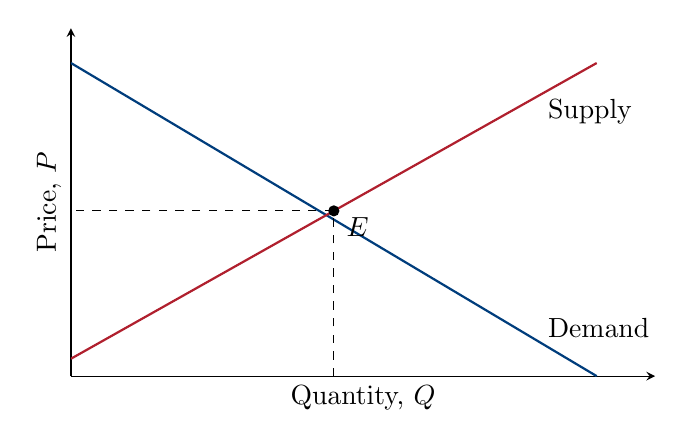
\begin{tikzpicture}
    \begin{axis}[
      width=9cm, height=6cm,
      xmin=0, xmax=10, ymin=0, ymax=10,
      xlabel={Quantity, $Q$}, ylabel={Price, $P$},
      axis lines=left, ticks=none,
      ]
      \addplot[wublue, thick] coordinates {(0,9) (9,0)};
      \addplot[wured, thick] coordinates {(0,0.5) (9,9)};
      \addplot[only marks, mark=*, mark size=1.8pt, black] coordinates {(4.5,4.75)};
      \draw[dashed] (axis cs:4.5,0) -- (axis cs:4.5,4.75) -- (axis cs:0,4.75);
      \node[anchor=west] at (axis cs:8,7.6) {Supply};
      \node[anchor=west] at (axis cs:8,1.4) {Demand};
      \node[anchor=north west] at (axis cs:4.55,4.85) {$E$};
      \node[anchor=east, font=\scriptsize] at (axis cs:0,4.75) {$P_E$};
      \node[anchor=north, font=\scriptsize] at (axis cs:4.5,0) {$Q_E$};
    \end{axis}
  \end{tikzpicture}
  \end{center}
  \centering \small
  Market equilibrium: the unique price/quantity pair at which demand equals supply, and both sides of the market are satisfied.
\end{frame}

\begin{frame}{Consumer and Producer Surplus}
  \begin{columns}[T]
    \begin{column}{0.5\textwidth}
      \begin{block}{Consumer surplus}
        The value consumers get from a good, above and beyond what they paid. Area below demand, above $P_E$.
      \end{block}
    \end{column}
    \begin{column}{0.5\textwidth}
      \begin{block}{Producer surplus}
        The profit producers earn, above and beyond their cost. Area above supply, below $P_E$.
      \end{block}
    \end{column}
  \end{columns}
  \begin{center}
  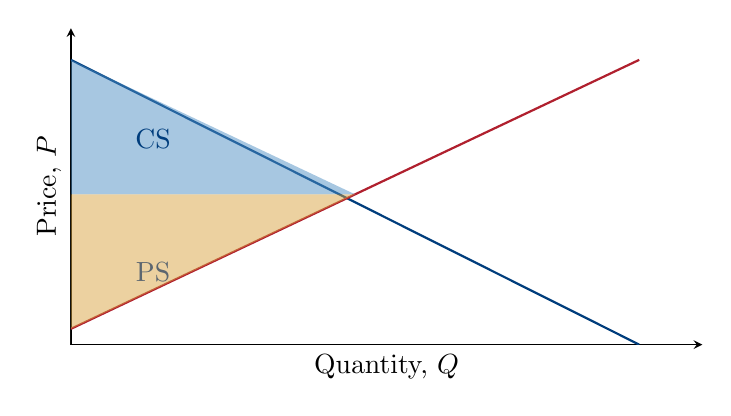
\begin{tikzpicture}
    \begin{axis}[
      width=9.6cm, height=5.6cm,
      xmin=0, xmax=10, ymin=0, ymax=10,
      xlabel={Quantity, $Q$}, ylabel={Price, $P$},
      axis lines=left, ticks=none,
      ]
      \addplot[wublue, thick] coordinates {(0,9) (9,0)};
      \addplot[wured, thick] coordinates {(0,0.5) (9,9)};
      \addplot[fill=wulight, draw=none, opacity=0.5] coordinates {(0,9) (4.5,4.75) (0,4.75)} \closedcycle;
      \addplot[fill=wuyellow, draw=none, opacity=0.5] coordinates {(0,0.5) (4.5,4.75) (0,4.75)} \closedcycle;
      \node[wublue] at (axis cs:1.3,6.5) {CS};
      \node[wugray] at (axis cs:1.3,2.3) {PS};
    \end{axis}
  \end{tikzpicture}
  \end{center}
\end{frame}

\begin{frame}{The First Fundamental Theorem of Welfare Economics}
  \begin{alertblock}{First Fundamental Theorem}
    \end{alertblock}
    The competitive equilibrium, where supply equals demand, maximizes total economic  efficiency. \\
  1st Welfare Theorem holds if (1) no externalities, (2) perfect competition [individuals and
firms are price takers], (3) perfect information, (4) agents are rational, then private
market equilibrium is Pareto efficient
  \begin{itemize}
    \item Total surplus just counts \texteuro{} --- it is blind to \emph{who} gets them.
    \item When these assumptions fail (market failures), government intervention can potentially raise --- not just redistribute --- total surplus.
  \end{itemize}

\end{frame}

\begin{frame}{Application: Rent Regulation in Vienna}
  
  \begin{itemize}
    \item About \textbf{21\%} of Vienna's rented apartments are subject to the \emph{Richtwertmietzins} price ceiling (currently \texteuro{}6.74/m\textsuperscript{2}), below the market rent.
    \item If this price is below the equilibrium price, what happens to apartment supply?
  \end{itemize}

 
\end{frame}

\begin{frame}{The Second Fundamental Theorem of Welfare Economics}

  \begin{alertblock}{Second Fundamental Theorem}
    \end{alertblock}
    Any Pareto-efficient allocation can be reached by (1) suitably redistributing initial endowments via \textbf{lump-sum} transfers, then (2) letting markets work freely.


  If this worked in practice, there would be \emph{no conflict} between efficiency and equity.
\end{frame}

\begin{frame}{Why the Second Theorem Fails in Practice}
  \begin{itemize}
    \item Lump-sum redistribution requires the government to observe individual \emph{characteristics} (need, ability) --- not just \emph{outcomes} (income, work status).
    \item In reality, the government usually cannot tell these apart, and must base taxes/transfers on observable behavior instead.
  \end{itemize}
 
\end{frame}

\begin{frame}{Social Welfare Functions: Utilitarian}
	With a utilitarian social welfare function, society’s goal is to maximize the sum of
	individual utilities:
	      \[SWF = U_1 + U_2 + \cdots + U_N\]
	The utilities of all individuals are given equal weight, and summed to get total social
	welfare \\
	If marginal utility of money decreases with income (satiation), utilitarian criterion
	values redistribution from rich to poor \\
	Taking $1$ for a rich person decreases his utility by a small amount, giving the $1$ to a
	poor person increases his utility by a large amount
   Transfers from rich to poor increase total utility

\end{frame}
\begin{frame}{Social Welfare Functions: Rawlsian}
Rawls (1971) proposed that society’s goal should be to maximize the well-being of its
worst-off member. The Rawlsian SWF has the form:
       \[SWF = \min(U_1, U_2, \ldots, U_N)\]
Since social welfare is determined by the minimum utility in society, social welfare is
maximized by maximizing the well-being of the worst-off person in society
(=maxi-min) \\
Rawlsian criterion is even more redistributive than utilitarian criterion: society wants
to extract as much tax revenue as possible from the middle and rich to make transfers
to the poor as large as possible

   
       
\end{frame}

\begin{frame}{Other Social Justice Principles}
  \begin{enumerate}
    \item \textbf{Commodity egalitarianism}: society should guarantee basic needs (education, health care, retirement) as rights; beyond that, distribution doesn't matter.
    \item \textbf{Equality of opportunity}: individuals should be compensated for circumstances beyond their control (family background, ability) --- but not for the consequences of their own choices.
    \item \textbf{Just deserts}: compensation should match contribution --- taxes should track the benefits an individual receives from government (a libertarian view).
  \end{enumerate}
  \vspace{0.3em}
  \centering \small
  None of these reduce cleanly to utilitarian or Rawlsian social welfare --- real policy debates mix all three.
\end{frame}

\begin{frame}{What Do People Actually Think Is Fair?}
 
  Saez \& Stantcheva (2016) surveyed \(\approx\)1{,}100 US respondents with hypothetical vignettes: two people have identical pre-tax and post-tax income --- who deserves a \texteuro{}1{,}000 tax break more?
  \begin{itemize}
 \item People favor redistribution if they feel inequalities are “unfair” but views on what is
 fair differ
 \item Redistribution supported when people don’t have control [education for children,
 health insurance for the sick]  
 \item Less support when people have some or full control [unemployment, being low
 income]
  \item Less support when people don’t “belong” (us vs. them)
 \end{itemize} 
  
  \srcnote{Saez, E.\ and Stantcheva, S.\ (2016), ``Generalized Social Marginal Welfare Weights for Optimal Tax Theory,'' \emph{American Economic Review}.}
\end{frame}

% =============================================================
 
 

% =============================================================


\begin{frame}[standout]
  Thank you!\\
  \vspace{0.5em}
  \small Questions and discussion
\end{frame}

\end{document}
